\chapter{Vorbereitung}
    \section{Aufbau eines Oszilloskop-Tastkopfes}
        Der Tastkopf dient als Verbindung zwischen dem Oszilloskop und der zu messenden Spannung. Es ist auch möglich ein Kabel zu verwenden, jedoch sind dann Widerstand und Kapazität bei der Messung undefiniert. Bei hohen Frequenzen wird dadurch das Messsignal verfälscht. Der Tastkopf kann die Spannung unter bekannten Bedingungen Messen.~\cite{tastkopf_deniz}
        Die Signalverarbeitung eines Tastkopfes kann mit passiven Bauelementen erfolgen oder durch eine aktive Schaltung. Wichtig ist das der Eingangswiderstand eines Tastkopfes möglichst groß und die Einkangskapazität möglichst klein ist, damit das Signal unverfälscht weitergegeben wird. Dabei gibt es viele verschiedene Tastköpfe mit eigenen Eigenschaften. Im Folgenden sind diese mit ihrem Aufbau aufgelistet.~\cite{tastkopf_wiki}

        \begin{enumerate}

        \item Standard-Tastkopf
            \begin{figure}[h!]
                \centering
                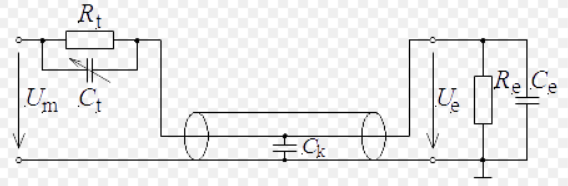
\includegraphics[]{111.PNG}
                \caption{Aufbau eines Standart Tastkopfes~\cite{tastkopf_standard}}
            \end{figure}

        \item Transmissions-Line-Tastkopf
            \begin{figure}[h!]
                \centering
                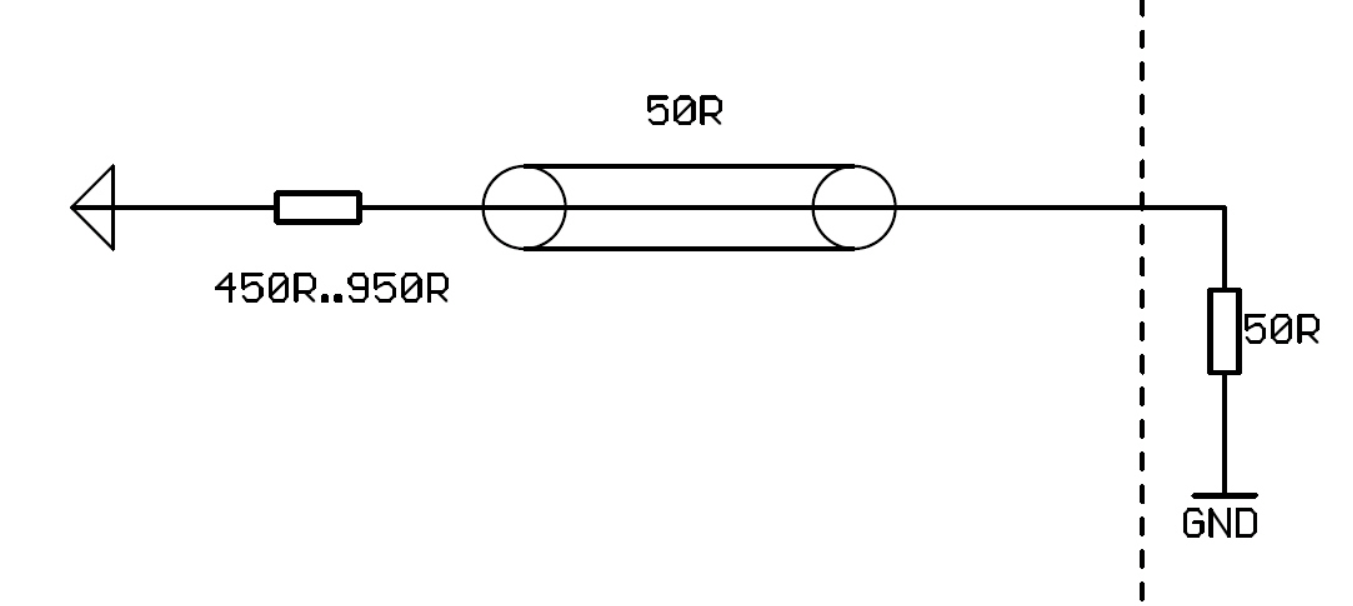
\includegraphics[width=0.5\linewidth]{112.PNG}
                \caption{Aufbau eines Transmission-Line-Tastkopfes~\cite{transmission_line_probe}}
            \end{figure}
        \newpage
        \item Aktiver Tastkopf
            \begin{figure}[h!]
                \centering
                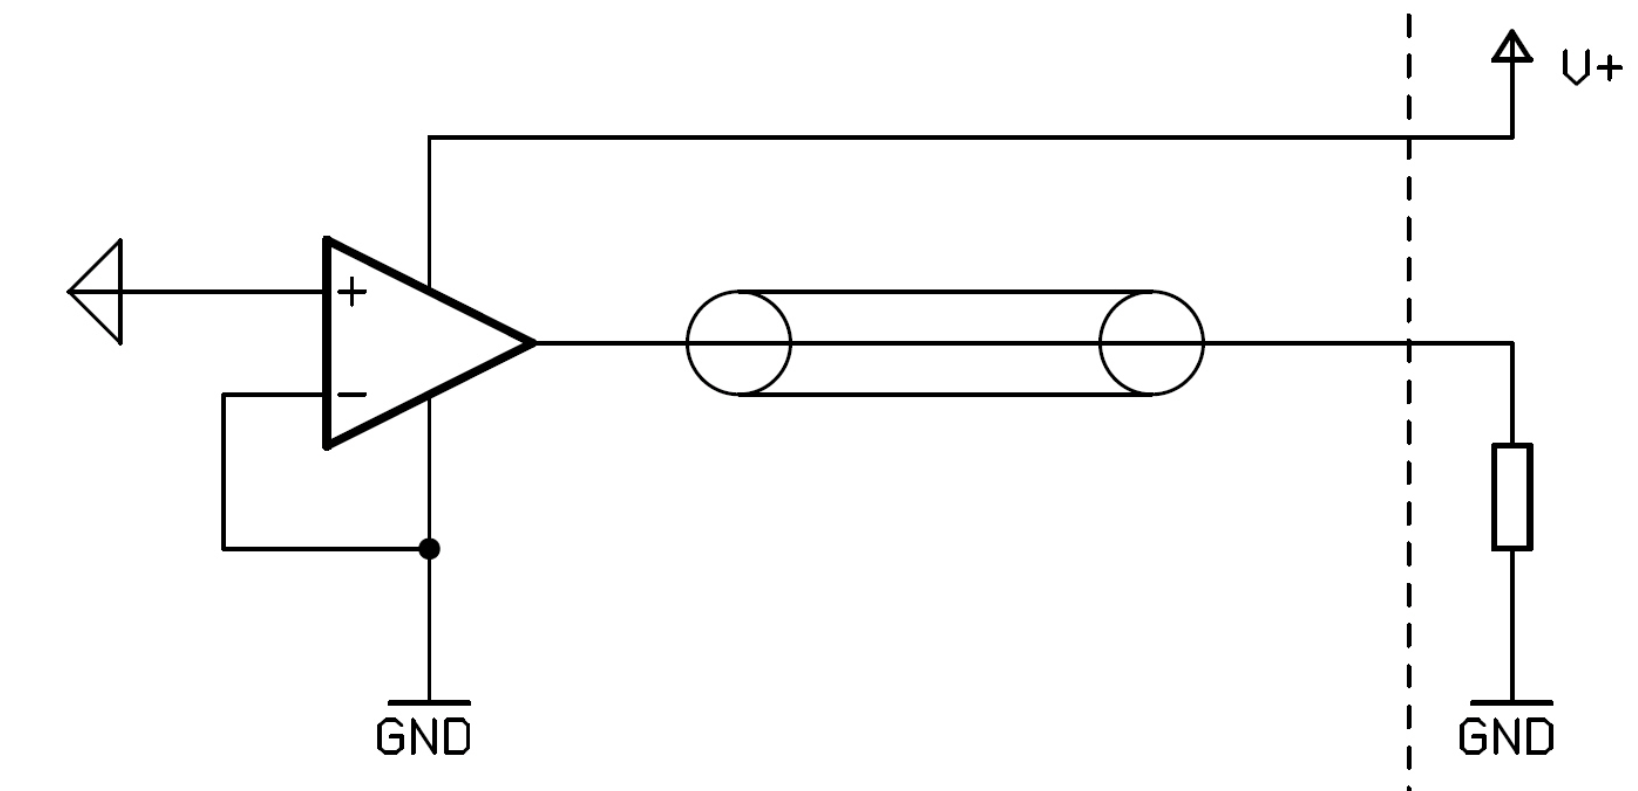
\includegraphics[width=0.5\linewidth]{113.PNG}
                \caption{Aufbau eines aktiven Tastkopfes~\cite{active_probe}}
            \end{figure}

        \item Differentieller Tastkopf
            \begin{figure}[h!]
                \centering
                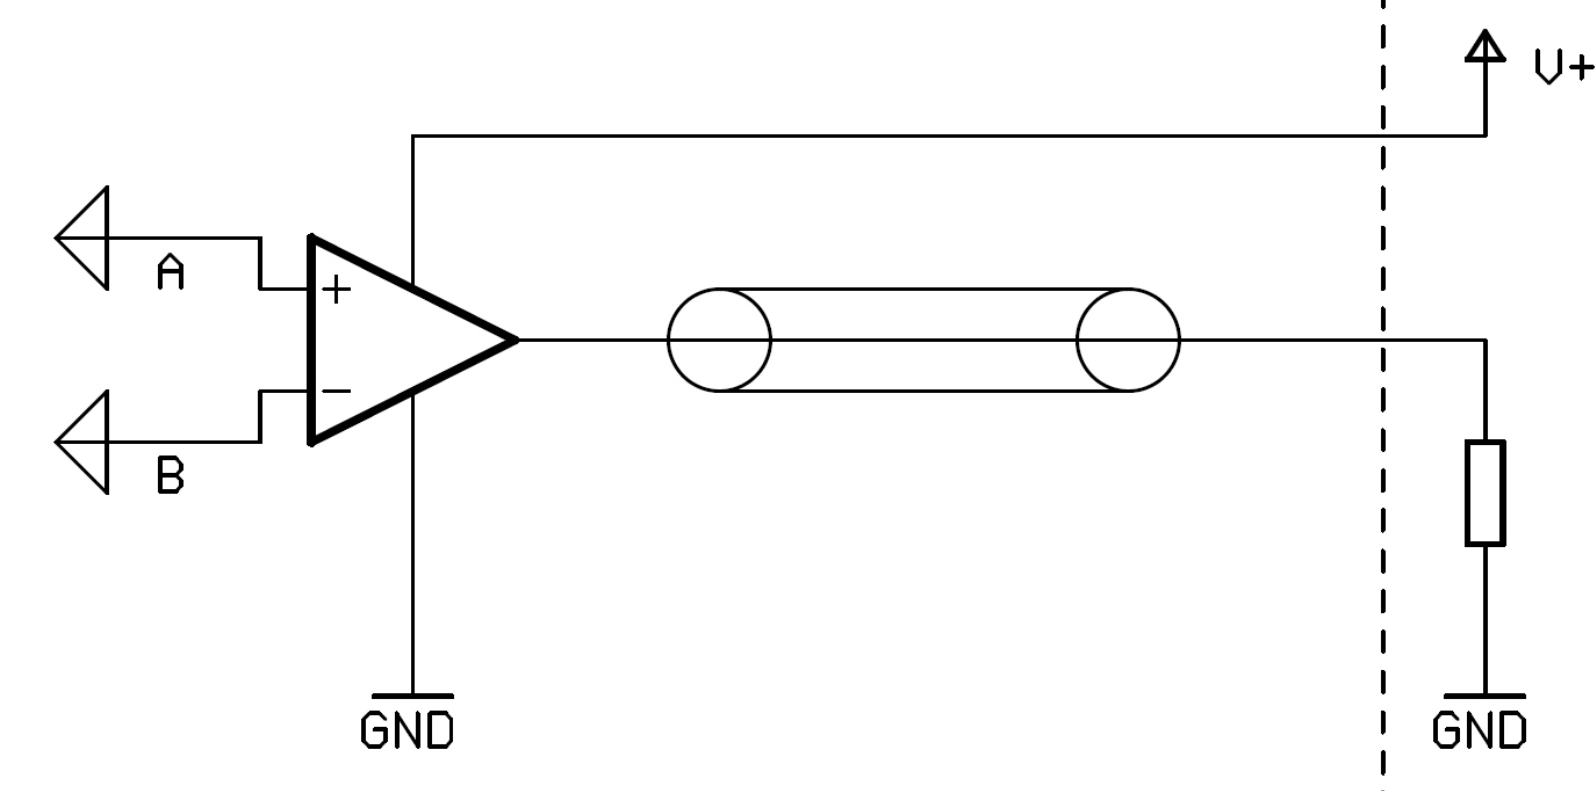
\includegraphics[width=0.5\linewidth]{114.PNG}
                \caption{Aufbau eines differentiellen Tastkopfes~\cite{differential_probe}}
            \end{figure}

        \end{enumerate}

        \begin{table}[h!]
            \centering
            \caption{Begriffserklärung für die einzelnen Buchstaben in den Abbildungen}
            \begin{tabular}{|c|c|}
                \hline
                $R_t$ & Tastkopfwiderstand\\ \hline \hline
                $C_t$ & Tastkopfkapazität \\ \hline
                $U_m$ & Spannungsmessung\\ \hline
                $C_K$ & Kabelkapazität\\ \hline
                $U_e$ & Eingangsspannung\\ \hline
                $R_e$ & Eingangswiderstand\\ \hline
                $C_e$ & Eingangskapazität\\ \hline
                Zahl mit R & Widerstand mit Zahlenwert \\ \hline
                GND & Ground (zu Erde)\\ \hline
                V & Spannung\\ \hline
            \end{tabular}
        \end{table}

